\documentclass[11pt]{article} 
\usepackage[T1]{fontenc}
\usepackage[french]{babel}
\usepackage[margin=1in]{geometry}
\usepackage{amssymb}
\usepackage{amsmath}
\usepackage{graphicx}
\usepackage{float}
\usepackage{enumitem}
\graphicspath{{figs/}}

\begin{document}

\title{TIPE 2025 : Modélsiation d'hystérésis}
\author{Pacôme Daval \and Maxime Brun \and Paul Brunot}
\date{\today}
\maketitle

\begin{figure}[H]
    \centering
    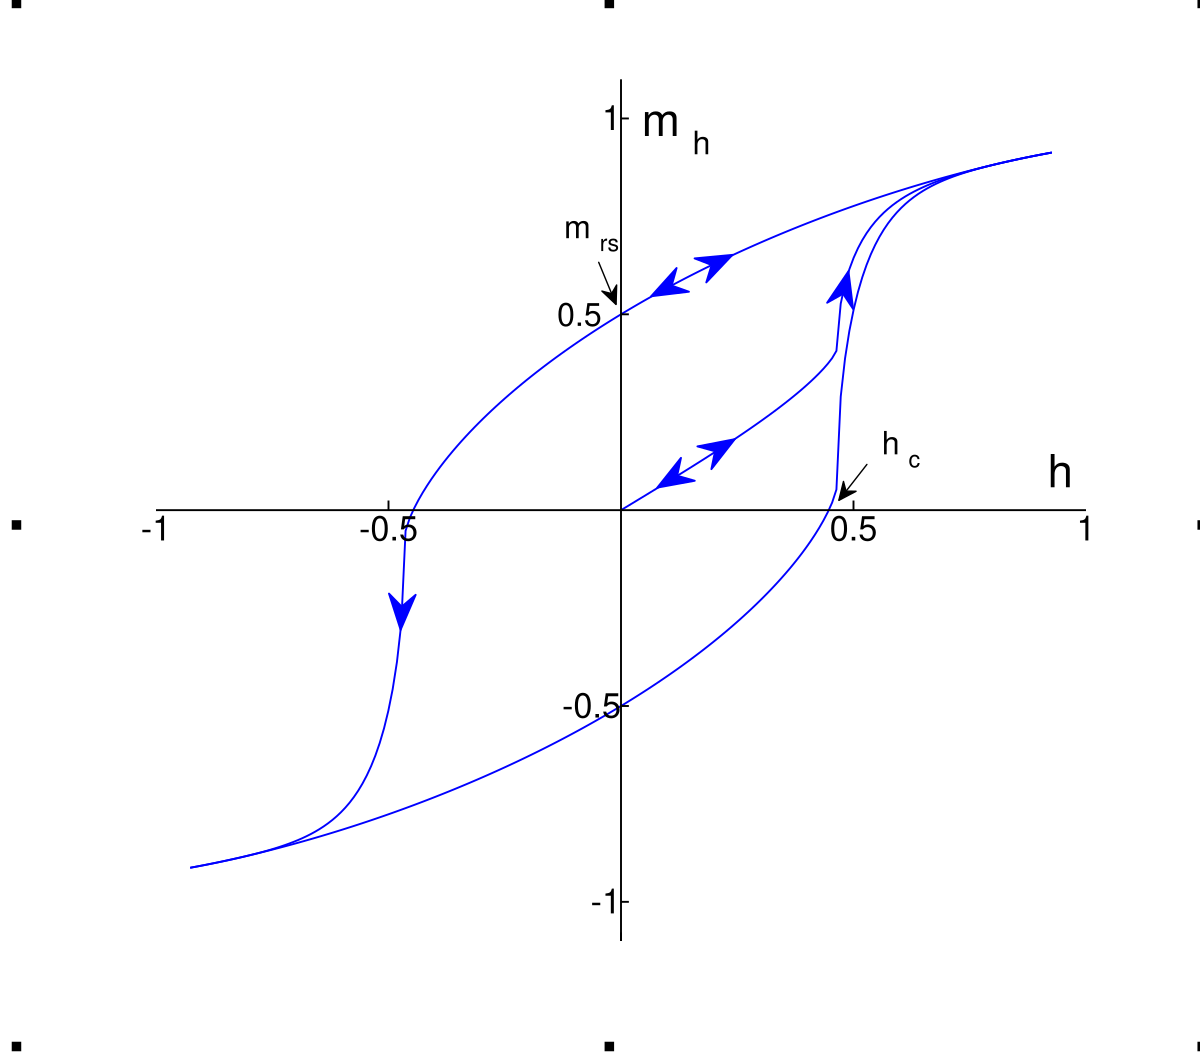
\includegraphics[width=0.5\textwidth]{Hysteresiscurve.png}
    \caption{Cycle d'hystérésis d'un matériau ferromagnétique.}
    \label{fig:hysteresis_title}
\end{figure}

\newpage

\tableofcontents
\newpage

\section{Introduction}

L'objectif inital de ce TIPE est d'un coté de modéliser le phénomène d'hystérésis en comparant les différentes
modèles préexistant et dans la mesure du possible comparer la modélisation avec les expériences faites.

\subsection{Définitions}
Avant tout, commençons par définir tous le vocabulaire qui va être utilisé en particulier ce qu'est un cycle d'hystérésis.
Comme cela est défini dans le \textit{Dictionnaire de l'Académie Française} : 
\begin{description}
    \item[Hystérésis :] Phénomène qui s'observe dans les réactions élastiques ou magnétiques de certains corps et qui consiste en un retard de l'effet sur la cause.
\end{description}

Ou globalement, l'évolution de l'état d'un système possède une dissymétrie en fonction de l'évolution d'une cause extérieure.
Cette définition un peu barbare, de prime abord, mais au fond exlique juste que l'état d'un système dépend directement de son état passé pour de mêmes conditions extérieures.



Ainsi; nous pouvons défnir ce qu'est un cycle d'hystérésis :
\begin{description}
    \item[Cycle d'hystérésis :] Lorsqu'on impose à la cause C des variations périodiques, l'hystérésis est responsable d'une forme particulière pour la 
    courbe E = f(C) appelée \textbf{cycle d'hystérésis}. Une valeur x peut donc avoir deux images y différentes.
\end{description}
Il est important de noter qu'un cycle d'hystérésis est la plupart du temps orienté pour connaitre précisément sont état.
\begin{figure}[H]
    \centering
    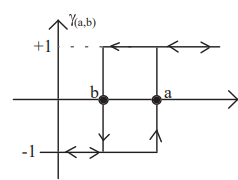
\includegraphics{Cycle_base.png}
    \caption{Cycle d'hystérésis}
    \label{fig:hysteresis_cycle_base}
\end{figure}

\subsection{Histoire}

C'est au milieu du 19ème siècle qu'un certains nombre scientifiques ont commencé à remarquer que
certaines machines possédant un noyau ferromagnétique présentaient des pertes d'énergie lors que cycles.



Mais c'est en 1881 que le physicien \textit{Sir James Alfred Ewing} fut le premier à utiliser le terme
d'hystérésis pour décrire le comportement de certains matériaux magnétiques au sein d'un champ magnétique.

Au cours du début du 20ème siècle, un grand nombre de découverte scientifiques sont faites autour du magnétisme
en particulier l'influence assez importante de la température pour des matériaux ferromagnétiques. 
En particulier \textit{Pierre Curie} qui met en évidence la présence d'une température à partir de laquelle
un matérieu ferromagnétique perd son magnétisme : la température de Curie.

C'est en 1935 que le physicien Allemand \textit{Ferenc Preisach} propose une première modélisation de ce phénomène concernant
les matériaux ferromagnétiques. Ce modèle est un des principaux modèles existant de nos jours pour modéliser les hysteresis.
Ce modèle sera abordé dans la suite de ce document, ainsi que ses caractéristiques et ses limites.

Le deuxième modèle fut quant à lui publié en 1969 par \textit{Robert Bouc} ingénieur au CEA, puis amélioré par 
\textit{Yi-Kwei Wen} en 1976. Ainsi, le modèle Bouc-Wen est aujourd'hui le modèle le plus adapté pour modéliser
les cycles d'hystérésis mais aussi le plus modelable pour l'appliquer à un grand nombre de sitations.

\begin{figure}[H]
    \centering
    \begin{minipage}{0.2\textwidth}
      \centering
      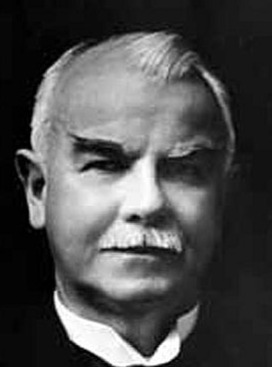
\includegraphics[width=\textwidth]{James_A_Ewing.jpg}
      \caption{Sir James Alfred Ewing}
    \end{minipage}
    \hspace{1in}
    \begin{minipage}{0.27\textwidth}
      \centering
      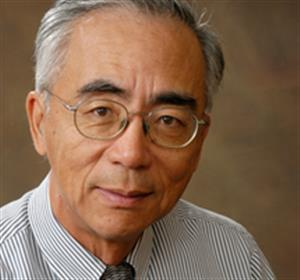
\includegraphics[width=\textwidth]{Yi-Wen.jpeg}
      \caption{Yi-Kwei Wen}
    \end{minipage}
  \end{figure}
  
\subsection{Utilisations}
Le phénomène d'hystérésis fut à l'origine théorisé pour les matériaux ferromagnétiques, mais il a, depuis,
été adapté dans un grand nombre de domaines. On peut aisni le retrouver dans la gestion thermique de batiments (chauffe eau),
dans l'étude des matériaux élastiques, composites, dans la mécanique des sols et des séismes, dans la gestion du chômage... 

\section{Modélisation}

Il existe aujourd'hui un certains nombre de modèles qui s'intéressent aux hystérésis. Cependant, il esy possible
de les regrouper en deux grandes catégories :
\begin{enumerate}
    \item Ceux basé sur un opérateur (\textbf{operator based model})
    \begin{itemize}
        \item Ils sont basés sur un opérateur non linéaire qui "garde mémoire" du passé pour déterminer l'état futur du système.
        \item C'est le cas du modèle de \underline{Preisach}
    \end{itemize}
    \item Les modèles différentiels (\textbf{differential based model})
    \begin{itemize}
        \item Ils sont basés sur des systèmes d'équations différentielles non-linéaires qui décrivent l'évolution du système en fonction du temps.
        \item C'est le cas du modèle de \underline{Bouc-Wen}
    \end{itemize}
\end{enumerate}


\subsection{Modèle de Preisach}
\subsection{Modèle de Bouc-Wen}

\section{Expérience}
\subsection{Matériaux ferromagnétiques}

\section{Comparaison}

\section{Conclusion}
\end{document}